% -*- latex -*-
%%%%%%%%%%%%%%%%%%%%%%%%%%%%%%%%%%%%%%%%%%%%%%%%%%%%%%%%%%%%%%%%
%%%%
%%%% This TeX file is part of the course
%%%% Introduction to Scientific Programming in C++/Fortran2003
%%%% copyright 2017-2023 Victor Eijkhout eijkhout@tacc.utexas.edu
%%%%
%%%% proto.tex : about prototypes and separate compilation
%%%%
%%%%%%%%%%%%%%%%%%%%%%%%%%%%%%%%%%%%%%%%%%%%%%%%%%%%%%%%%%%%%%%%

In this chapter you will learn techniques
that you need for modular program design.

\Level 0 {Include files}

You have seen the \lstinline+#include+ directive
in the context of \indextermp{header file}
of the \ac{STL}, most notably the \lstinline{iostream} header.
But you can include arbitrary files, including your own.

To include files of your own, use a slightly different syntax:
\begin{lstlisting}
#include "myfile.cpp"
\end{lstlisting}
(The angle bracket notation usually only works
with files that are in certain system locations.)
This statement acts as if the file
is literally inserted at that location of the source.

\begin{figure}[ht]
  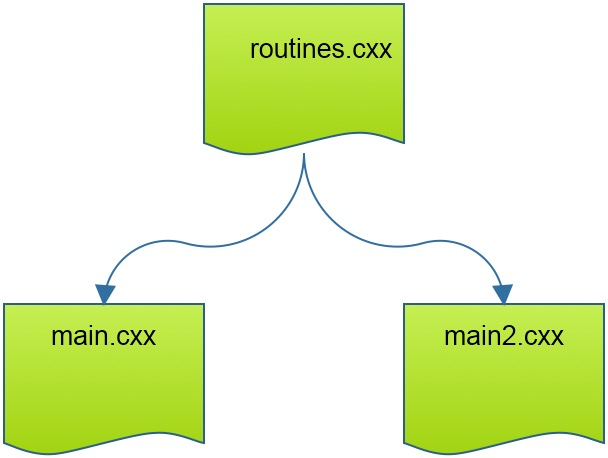
\includegraphics[scale=.4]{twomains}
  \caption{Using an include file for two main programs}
  \label{fig:twomains}
\end{figure}
This mechanism gives an easy solution to the problem
of using some functions or classes in more than one main program;
see figure~\ref{fig:twomains}.

The problem with this approach is that building the two main programs
takes a time (roughly) equal to
the sum of the compile times of the main programs
and \textbf{twice} the compile time of the included file.
Also, any time you change the included file
you need to recompile the two main programs.

In a better scenario you would compile all three files once,
and spend some little extra time tie-ing it all together.
We will work towards this in a number of steps.

\Level 0 {Function declarations}
\label{sec:proto}

In most of the programs you have written in this course, you put any
functions or classes above the main program, so that the compiler
could inspect the definition before it encountered the use. However,
the compiler does not actually need the whole definition, say of a
function: it is enough to know its name, the types of the input
parameters, and the return type.

Such a minimal specification of a function is known as
\indextermbusdef{function}{prototype}; for instance
\begin{lstlisting}
int tester(float);
\end{lstlisting}

\begin{block}{Forward declarations, 1}
  \label{sl:forward-proto1}
  A first use of declarations is \indextermp{forward declaration}.

  Some people like defining functions after the main:
\begin{multicols}{2}
\begin{lstlisting}
  int f(int);
  int main() {
    f(5);
  };
  int f(int i) {
    return i;
  }
\end{lstlisting}
\columnbreak
versus before:
\begin{lstlisting}
int f(int i) {
  return i;
}
int main() {
  f(5);
};
\end{lstlisting}
\end{multicols}
\end{block}

\begin{block}{Forward declarations, 2}
  \label{sl:forward-proto2}
  You also need forward declaration for mutually recursive functions:
\begin{lstlisting}
int f(int);
int g(int i) { return f(i); }
int f(int i) { return g(i); }
\end{lstlisting}
\end{block}

Declarations are useful if you spread your program over multiple
files. You would put your functions in one file
and the main program in another.

\begin{multicols}{2}  
\begin{lstlisting}
// file: def.cpp
int tester(float x) {
  .....
}
\end{lstlisting}
\vfill\columnbreak
\begin{lstlisting}
// file : main.cpp
int main() {
  int t = tester(...);
  return 0;
}
\end{lstlisting}
\end{multicols}

In this example a function \n{tester}
is defined in a different file from the main program, so we need to
tell \n{main} what the function looks like in order for the main
program to be compilable:

\begin{lstlisting}
// file : main.cpp
int tester(float);
int main() {
  int t = tester(...);
  return 0;
}
\end{lstlisting}

Splitting your code over multiple
files and using
\indextermsub{separate}{compilation} 
is good software engineering practice for a number of
reasons. 
\begin{enumerate}
\item If your code gets large, compiling only the necessary files cuts
  down on compilation time.
\item Your functions may be useful in other projects, by yourself or
  others, so you can reuse the code without cutting and pasting it
  between projects.
\item It makes it easier to search through a file without being
  distracted by unrelated bits of code.
\end{enumerate}

\begin{slide}{Declarations for separate compilation}
\label{sl:separate-proto}
\begin{multicols}{2}  
\begin{lstlisting}
// file: def.cpp
int tester(float x) {
  .....
}
\end{lstlisting}
\vfill\columnbreak
\begin{lstlisting}
// file : main.cpp
int tester(float);

int main() {
  int t = tester(...);
  return 0;
}
\end{lstlisting}
\end{multicols}
\end{slide}

(However, you would not do things like this in practice. See 
section~\ref{sec:headerfile} about header files.)

\Level 1 {Separate compilation}
\index{object file|see{file, object}}

\begin{block}{Compiling and linking}
  \label{sl:compile-link}
  Your regular compile line
\begin{verbatim}
icpc -o yourprogram yourfile.cc
\end{verbatim}
  actually does two things: compilation, and linking. You can do those
  separately:
  \begin{enumerate}
  \item First you compile
\begin{verbatim}
icpc -c yourfile.cc
\end{verbatim}
  which gives you a file \n{yourfile.o}, a so-called
  \indextermsub{object}{file}; and
  \item Then you use the compiler as \indexterm{linker} to give you
    the \indextermsub{executable}{file}:
\begin{verbatim}
icpc -o yourprogram yourfile.o
\end{verbatim}
  \end{enumerate}
\end{block}

In this particular example you may wonder what the big deal is.
That will become clear if you have multiple source files: now you
invoke the compile line for each source, and you link them only once.

\begin{block}{Dealing with multiple files}
  \label{sl:link-multiple}
  Compile each file separately, then link:
\begin{verbatim}
icpc -c mainfile.cc
icpc -c functionfile.cc
icpc -o yourprogram mainfile.o functionfile.o
\end{verbatim}  
\end{block}

At this point, you should learn about the \indexterm{Make} tool for
managing your programming project.

\Level 1 {Header files}
\label{sec:headerfile}
\label{sec:hfile}

Even better than writing the declaration every time you need the
function is to have a \indexterm{header file}:

%%packtsnippet hfile

\begin{block}{Declarations and header files}
  \label{sl:proto-header}
  Using a header file with function declarations.
  \begin{multicols}{2}
    Header file contains only declaration:
    \columnbreak
\begin{lstlisting}
// file: def.h
int tester(float);
\end{lstlisting}
\end{multicols}

The header file gets included both in the definitions file and the
main program:
\begin{multicols}{2}  
\begin{lstlisting}
// file: def.cpp
#include "def.h"
int tester(float x) {
  .....
}
\end{lstlisting}
\vfill\columnbreak
\begin{lstlisting}
// file : main.cpp
#include "def.h"

int main() {
  int t = tester(...);
  return 0;
}
\end{lstlisting}
\end{multicols}
What happens if you leave out the \lstinline$#include "def.h"$ in both cases?
\end{block}

Having a header file is an important safety measure:
\begin{itemize}
\item Suppose you change your function definition, changing its return
  type:
\item The compiler will complain when you compile the definitions
  file;
\item So you change the declaration in the header file;
\item Now the compiler will complain about the main program, so you
  edit that too.
\end{itemize}

It is necessary to include the header file in the main program. It is
not strictly necessary to include it in the definitions file, but
doing so means that you catch potential errors: if you change the
function definitions, but forget to update the header file, this is
caught by the compiler.

%%packtsnippet end

\begin{remark}
  By the way, why does that compiler even recompile the main program,
  even though it was not changed? Well, that's because you used a
  \indexterm{makefile}. See \CARPref{tut:gnumake}.
\end{remark}
\begin{remark}
  Header files were able to catch more errors in~C than they do
  in~C++. With polymorphism of functions, it is no longer an error to
  have 
\begin{lstlisting}
// header.h
int somefunction(int);
\end{lstlisting}
and
\begin{lstlisting}
#include "header.h"

int somefunction( float x ) { .... }
\end{lstlisting}
\end{remark}

\Level 1 {C and C++ headers}

You have seen the following syntaxes for including header files:
\begin{lstlisting}
#include <header.h>
#include "header.h"
\end{lstlisting}
The first is typically used for system files, with the second
typically for files in your own project. There are some header files
that come from the C~standard library such as \n{math.h}; the
idiomatic way of including them in C++ is
\begin{lstlisting}
#include <cmath>
\end{lstlisting}

\Level 0 {Declarations for class methods}
\label{sec:class-header-file}

Section~\ref{sec:class-decl-defn} explained how you can split a
class declaration from its definition.
You can then put the declaration in a header file that
you include where is a class is used,
while the definitions get compiled only once,
and linked in when the executable of your program is built.

\begin{block}{Class declarations}
  \label{sl:class-proto}
  Header file:
  \verbatimsnippet{classheaderdefine}

  Implementation file:
  \verbatimsnippet{classheaderimpl}
\end{block}

\begin{block}{Data members in proto}
  \label{sl:class-proto-private}
  Data members, even private ones, need to be in the header file:
  \lstset{style=snippetcode}
\begin{lstlisting}
class something {
private:
  int localvar;
public:
  // declaration:
  double somedo(vector);
};
\end{lstlisting}
Implementation file:
\begin{lstlisting}
// definition
double something::somedo(vector v) {
   .... something with v ....
   .... something with localvar ....
};
\end{lstlisting}
\end{block}

\begin{review}
  \label{rev:proto-c-cpp}
  For each of the following answer: is this a valid function
  definition or function declaration.
  \begin{itemize}
  \item \lstinline+int foo();+
  \item \lstinline+int foo() {};+
  \item \lstinline+int foo(int) {};+
  \item \lstinline+int foo(int bar) {};+
  \item \lstinline+int foo(int) { return 0; };+
  \item \lstinline+int foo(int bar) { return 0; };+
  \end{itemize}
\end{review}

\Level 0 {More}

\Level 1 {Header files and templates}

See section~\ref{sec:templ-header}.

\Level 1 {Namespaces and header files}
\label{sec:namespace-header}

Namespaces
(see chapter~\ref{ch:namespace})
are convenient, but they carry a danger in that they may define
functions without the user of the namespace being aware of it.

Therefore, one should never put \indexc{using namespace} in a header
file.

\Level 1 {Global variables and header files}
\label{ex:globalvar}

If you have a variable that you want known everywhere, you can make it
a \indextermsub{global}{variable}:
\begin{lstlisting}
int processnumber;
void f() {
  ... processnumber ...
}
int main() {
  processnumber = // some system call
};
\end{lstlisting}
It is then defined in the main program and any functions defined in your program file.

Warning: it is tempting to define variables global but this is a
dangerous practice; see section~\ref{sec:namespace-practice}.

If your program has multiple files, you should not put `\n{int processnumber}'
in the other files, because that would create a new variable, that is
only known to the functions in that file. Instead use:
\begin{lstlisting}
extern int processnumber;
\end{lstlisting}
which says that the global variable \n{processnumber} is defined in
some other file.

What happens if you put that variable in a
%
\emph{header file}\index{header file!and global variables}%
\index{variable!global!in header file}%
? Since the
%
\emph{preprocessor}\index{preprocessor!and header files}%
\index{header file!treatment by preprocessor}
acts as if the header is textually inserted, this again leads to
a separate global variable per file. The solution then is more
complicated:
\begin{lstlisting}
//file: header.h
#ifndef HEADER_H
#define HEADER_H
#ifndef EXTERN
#define EXTERN extern
#fi
EXTERN int processnumber
#fi

//file: aux.cc
#include "header.h"

//file: main.cc
#define EXTERN
#include "header.h"
\end{lstlisting}
(This sort of preprocessor magic is discussed in chapter~\ref{ch:cpp}.)

This also prevents recursive inclusion of header files.

\Level 0 {Modules}
%%packtsnippet module
\label{sec:module}

The \cppstandard{20} standard is taking a different approach
to header files, through the introduction of \indextermdefp{module}.
\begin{fortranbook}
  (Fortran90 already had this for a long time; see chapter~\ref{ch:modulef}.)
\end{fortranbook}
This largely dispenses with the need for
header files included through the \ac{CPP}.
However, the \ac{CPP} may still be needed for other purposes.

\Level 1 {Program structure with modules}

Using modules, the \indexpragma{include} directive is no longer needed;
instead, the \indexcdef{import} keyword indicates what module is to be used
in a (sub)program:
%
\verbatimsnippet{mainwithmod}

The module is in a different file; the
\indexcdef{export} keyword,
followed by \indexcdef{module} defines the name of the module.
This file can then have any number of functions;
only the ones with the \indexc{export} keyword will be
visible in a program that imports the module.
%
\verbatimsnippet{modformain}

\Level 1 {Implementation and interface units}

A module can have a leveled structure, by using names with a
\lstinline{module:partition} structure.

This makes it possible to have separate
\begin{itemize}
\item Interface partitions, that define the interface to the using program; and
\item Implementation partitions, that contain the code that needs to
  be shielded from the user.
\end{itemize}

Here is an implementation partition; there is no \indexc{import} keyword
because this functionality is internal:
%
\verbatimsnippet{modhelper}

Here is an interface partition, which uses the internal function,
and exports a different function:
%
\verbatimsnippet{modintface}

%%packtsnippet end

\Level 1 {More}

Importable headers:
\begin{lstlisting}
import <header.h>
import "header.h"
\end{lstlisting}

Import declarations have to come before other module specifications,
whether import or export of modules or functions.

You can export variables, namespaces.
